% Created 2016-05-25 on. 16:55
\documentclass[11pt]{article}
\usepackage[utf8]{inputenc}
\usepackage[T1]{fontenc}
\usepackage{fixltx2e}
\usepackage{graphicx}
\usepackage{longtable}
\usepackage{float}
\usepackage{wrapfig}
\usepackage{rotating}
\usepackage[normalem]{ulem}
\usepackage{amsmath}
\usepackage{textcomp}
\usepackage{marvosym}
\usepackage{wasysym}
\usepackage{amssymb}
\usepackage{capt-of}
\usepackage{hyperref}
\tolerance=1000
\usepackage{minted}
\usepackage{tikz}
\usepackage{parskip}
\usepackage{color}
\usepackage{listings}
\usepackage{grffile}
\usepackage{xcolor}
\hypersetup{
colorlinks,
linkcolor={red!50!black},
citecolor={blue!50!black},
urlcolor={blue!80!black}
}
\usepackage[inline]{enumitem}
\usepackage{tikz,graphics,graphicx}
\usetikzlibrary{decorations.shapes,arrows,decorations.pathreplacing,decorations.pathmorphing,backgrounds}
\usetikzlibrary{decorations.pathmorphing}
\usetikzlibrary{shapes.geometric}
\usepackage{setspace}%% The linestretch
\singlespacing
\usepackage[format=hang,indention=0cm,singlelinecheck=true,justification=raggedright,labelfont={normalsize,bf},textfont={normalsize}]{caption} %
\usepackage{vmargin}
\setpapersize{A4}
\setmarginsrb{2.5cm}{1cm}% links, oben
{2.5cm}{2cm}% rechts, unten
{12pt}{30pt}% Kopf: Höhe, Abstand
{12pt}{30pt}% Fuß: Höhe, AB
\usepackage{upquote}
%  use straight quotes when printing a command in minted
\AtBeginDocument{%
\def\PYZsq{\textquotesingle}%
}
\setlength{\parindent}{0pt}
\setlength{\parskip}{\baselineskip}
\usepackage{minted}
\definecolor{mintedbackground}{rgb}{0.95,0.95,0.95}
\newminted{common-lisp}{fontsize=\footnotesize}
\author{Martin Jakt, Alexander Jueterbock\thanks{Nord University, Norway}}
\date{\textbf{PhD course: High throughput sequencing of non-model organisms}}
\title{\textbf{Mapping and Variant Calling} (June 2016)}
\hypersetup{
 pdfkeywords={},
  pdfsubject={},
  pdfcreator={Emacs 24.5.1 (Org mode 8.3beta)}}
\begin{document}

\maketitle
\tableofcontents









Once you have assembled a draft genome, you can map your reads against it
and identify potential read variants, like SNPs (Single Nucleotide
Polymorphisms) and InDels (Insertions and Deletions). The library that
you sequenced in this course is likely to represent a single diploid
individual. Read variants, thus, occur at loci that differed between
the mother and the father of this individual. Read variants become
interesting when they are associated with certain environmental
factors or phenotypes. This, however, requires sequencing several
individuals of differing phenotypes or obtained from several  
environments.

\section{Mapping with Bowtie2}
\label{sec-1}
Mapping next-generation sequencing data against genomes requires very high
performance algorithms that must balance the accuracy of the mapping with the
time taken. This is an interesting problem to work on and a rather large
number of different applications have been developed. 
To map reads against the assembled draft genome, we will use \href{http://bowtie-bio.sourceforge.net/bowtie2/index.shtml}{Bowtie2}.
Bowtie2 defaults to finding global alignments (no soft-clipping of
terminal bases) and it allows for gaps in the alignment, thereby
increasing mapping accurracy (\href{http://www.nature.com/nrg/journal/v15/n11/full/nrg3803.html}{Schlotterer \emph{et al}. (2014) \emph{Nature
Reviews Genetics}}). 

A number of aligners have been written to either compensate or make use of
the specific properties of sequence data obtained using different
technologies. For example the aligner \href{https://www.google.no/url?sa=t&rct=j&q=&esrc=s&source=web&cd=5&ved=0CD4QFjAE&url=https\%3A\%2F\%2Fgithub.com\%2Fiontorrent\%2FTMAP&ei=1u07VZCXFYGqywPBz4DoDg&usg=AFQjCNE3vZXuQ1ygljhBcrozKj_nBU84TQ&sig2=u5_YVYBE904ay-9oLUuMOQ&bvm=bv.91665533,d.bGQ}{TMAP} was specifically
designed to be used with Ion Torrent data which has problems with resolving
homopolymer lengths accurately. Similarly there are specific aligners that
handle SoliD color-space data which cannot be effectively aligned as
nucleotide sequences. In this tutorial we will make use of Bowtie2 as it is
one of the most commonly used aligners that balances speed, accuracy and
memory requirements. My current favourite aligner is the \href{http://bioinformatics.oxfordjournals.org/content/early/2012/10/25/bioinformatics.bts635}{STAR aligner}, which
was designed to align RNA sequences to genomic locations; it is rather
accurate and very fast, but requires far more memory to run than bowtie/bowtie2.
An alternative aligner that is also widely used is the \href{http://bio-bwa.sourceforge.net/}{BWA} aligner. You can
find an unpublished comparison of mapping performance \href{http://genomespot.blogspot.no/2014/11/dna-aligner-accuracy-bwa-bowtie-soap.html}{here}, a benchmarking of
9 mapping tools \href{http://bmcbioinformatics.biomedcentral.com/articles/10.1186/1471-2105-14-184}{here} and a more in-depth look at mapping RNA sequences to genomes \href{http://www.nature.com/nmeth/journal/v10/n12/full/nmeth.2722.html}{here}.

\subsection{The mapping commands}
\label{sec-1-1}

What you need for mapping are two sequence files, one containing the
quality-trimmed reads (fastq format) and the other containing the draft genome
(in the fasta format).

Create a new folder named \texttt{Mapping} (with \texttt{mkdir}) and copy the two
sequence files into it (with \texttt{cp}). For example for the assembly made using
IonTorrent data:

\begin{minted}[fontsize=\scriptsize,bgcolor=lightgray,linenos]{sh}
mkdir Mapping

cp GenomeAssembly/IonTorrentDeNovoAssembly_assembly/IonTorrentDeNovoAssembly_d_results/\
IonTorrentDeNovoAssembly_out.unpadded.fasta \
Mapping/

cp RAWREADS_trimmed_trimmed.fq \
Mapping/

cd Mapping
\end{minted}


Here the \texttt{RAWREADS\_trimmed\_trimmed.fq} refer to the IonTorrent reads after
quality trimming using TrimGalore. Here we are simply making copies of the
various files in different locations for performing different analyses. This is simple to describe and
understand, but is not a particularly good way to organise your files, both
because it wastes disk space\footnote{In some modern file systems that make use of Copy-On-Write,
there won't actually be any copying of the data unless one of the
files is modified.} and (more seriously) it makes it
easy to end up with files with the same names, but with slightly different
content\footnote{How to handle lots of files created by various versions of
data flows or pipelines is not a simple problem and there are many
systems that have been developed to address such problems. This comes
under the general heading of version control systems, and is outside
the scope of this course. In general though, it is wise to follow rule
number one of database design: 'never store a piece of information in
more than one location'. I.e. don't copy stuff around like we are
doing here.}.

In the Mapping folder, we first create an index for the reference genome using the
following command (enter the folder using \texttt{cd} before calling this command) :

\begin{minted}[fontsize=\scriptsize,bgcolor=lightgray,linenos]{sh}
bowtie2-build -f IonTorrentDeNovoAssembly_out.unpadded.fasta GENOMENAME
\end{minted}

You should change \texttt{GENOMENAME} to something that is suitable for your data.

Now, to align the trimmed reads against the genome, use the following command:

\begin{minted}[fontsize=\scriptsize,bgcolor=lightgray,linenos]{sh}
nohup bowtie2 -p 1 \
-q \
--phred33 \
--sensitive \
--no-unal \
--al-gz FILE_Aligned.fq.gz \
--un-gz FILE_Unaligned.fq.gz \
--met-file MetricsFile.txt \
-x GENOMENAME \
-U RAWREADS_trimmed_trimmed.fq \
-S MAPPEDREADS.sam >Logfile.log &
\end{minted}

Here an overview of the meaning of the used options:


\begin{description}
\item[{\texttt{-p 1}}] Causes Bowtie 2 to use a single thread.
Depending on the number of users and libraries we will  probably increase this.
\item[{\texttt{-q}}] Informs the program that the reads to map are saved in fastq files.
\item[{\texttt{-{}-phred33}}] Sets the quality encoding of the fastq files to  "Phred+33".
\item[{\texttt{-{}-sensitive}}] sets several options at once regarding the seeding and other adjustments.
\item[{\texttt{-{}-no-unal}}] Suppress SAM records for reads that do not align.
\item[{\texttt{-{}-al-gz}}] Write unpaired reads that align at least once to to the specified file.
\item[{\texttt{-{}-un-gz}}] Write unpaired reads that failed to align to the specified file.
\item[{\texttt{-{}-met-file}}] Write bowtie2 metrics to Metricsfile.txt.
\item[{\texttt{-x}}] Specifies the name of the genome.
\item[{\texttt{-U}}] Specify the unpaired reads to align (can contain a comma-separated list of several fq files).
\item[{\texttt{-S}}] Specify the sam file to which the alignment shall be saved.
\end{description}

You can't set the exact number of mismatches in the seed, but you can
adjust the mismatch penalty.  

The program should run no longer than 10-20 mins. The resulting output file will be
in the SAM format. For a detailed description of this format, see \href{https://samtools.github.io/hts-specs/SAMv1.pdf}{here}.

To map the Illumina data we follow a similar procedure; however, we need to
modify the call to \texttt{bowtie2} as the Illumina data is paired ended. To find
out how we can do this, we can run \texttt{bowtie2} without any arguments or
specifying the \texttt{-{}-help} option. This will
print out the usage information. Knowing how to read usage information is one
of the most important things you can do as you'll then be able to run most
applications without relying on others. If you do this, you'll see something
like this:

\begin{minted}[fontsize=\scriptsize,bgcolor=lightgray,linenos]{sh}
bowtie2 --help
Bowtie 2 version 2.1.0 by Ben Langmead (langmea@cs.jhu.edu, www.cs.jhu.edu/~langmea)
Usage: 
  bowtie2 [options]* -x <bt2-idx> {-1 <m1> -2 <m2> | -U <r>} [-S <sam>]

  <bt2-idx>  Index filename prefix (minus trailing .X.bt2).
             NOTE: Bowtie 1 and Bowtie 2 indexes are not compatible.
  <m1>       Files with #1 mates, paired with files in <m2>.
             Could be gzip'ed (extension: .gz) or bzip2'ed (extension: .bz2).
  <m2>       Files with #2 mates, paired with files in <m1>.
             Could be gzip'ed (extension: .gz) or bzip2'ed (extension: .bz2).
  <r>        Files with unpaired reads.
             Could be gzip'ed (extension: .gz) or bzip2'ed (extension: .bz2).
  <sam>      File for SAM output (default: stdout)

  <m1>, <m2>, <r> can be comma-separated lists (no whitespace) and can be
  specified many times.  E.g. '-U file1.fq,file2.fq -U file3.fq'.

Options (defaults in parentheses):

 Input:
  -q                 query input files are FASTQ .fq/.fastq (default)
  --qseq             query input files are in Illumina's qseq format
.... more options
\end{minted}


Let us consider the top lines first. This is the basic usage information
that tells you the arguments you need to specify and their order.

\begin{minted}[fontsize=\scriptsize,bgcolor=lightgray,linenos]{sh}
Usage: 
  bowtie2 [options]* -x <bt2-idx> {-1 <m1> -2 <m2> | -U <r>} [-S <sam>]
\end{minted}

Things contained in square brackets \texttt{[stuff in square brackets]} denote
optional arguments. So, the above (\texttt{bowtie2 [options] ...}) indicates that optional options (specified
with \texttt{-} or \texttt{-{}-}) should be specified before other arguments. After these
options (of which there may be none) you should specify the value of the \texttt{-x}
option. Looking down, you can see that \texttt{<bt2-idx>}, is a placeholder for
the name of the index that you built using \texttt{bowtie2} in the
previous section. If you have assembled a genome from the Illumina data on
its own this will be a different index file based on a different assembly
sequence, so we will need to change this value.

The next section of the usage line is contained in squiggly brackets (usually
referred to as braces) indicating that you have a choice of two or more
alternatives. These alternatives are seperated by the pipe (\texttt{|}) character
which in computing languages is usually taken to mean 'or'. So the section 
\texttt{\{-1 <m1> -2 <m2> | -U <r>\}} reads as 'either specify the values of \texttt{-1} and
\texttt{-2} or the value of \texttt{-U}. Looking at the explanation further down, you can
see that \texttt{<m1>} and \texttt{<m2>} refer to mate or paired sequences, whereas \texttt{<r>}
refers to unpaired reads. The last section simply specifies to which file we
wish to write the output; if you don't specify this, it will simply be
written to the terminal (i.e. \texttt{STDOUT}). This is useful, because we can then
pipe the data to other applications in a single command.

So reading the usage line (also known as the synopsis) we can design our
command line. If our paired reads are in files
\texttt{RAWREADS\_fw\_trimmed\_trimmed.fq} and 
\texttt{RAWREADS\_rv\_trimmed\_trimmed.fq}, and the index for our assembly genome is in 
\texttt{GENOMENAME.X.bt2}, the command without any of the optional options would be:

\begin{minted}[fontsize=\scriptsize,bgcolor=lightgray,linenos]{sh}
bowtie2 -x GENOMENAME -1 RAWREADS_fw_trimmed_trimmed.fq\
-2 RAWREADS_rv_trimmed_trimmed.fq -S MAPPED.sam
\end{minted}

Here we haven't specifed any of the options we used for the IonTorrent data
above and the program will simply use the default options. To see what the
default options are you should read the rest of the help section that is
printed out when you run \texttt{bowtie2} without any arguments. You can probably
use most of the options as we used above, though you should not assume this.

Given that the Illumina data is paired end sequence data you should pay
special attention to the Paired-end section of the help text. In particular
consider the values of \texttt{-I} and \texttt{-X} and whether the default options are
reasonable for your libraries.

\subsection{Running the commands in a script for posterity}
\label{sec-1-2}
As was emphasised in the section on Unix tools for bioinformatics, you
really shouldn't type these commands directly into a terminal
window. It's too easy to make a mistake when you have to specify many
options, and you will not have a record of the command that you
actually used. Instead we will write the commands into a text file and
ask the shell (in this case bash\footnote{bash stands for Bourne Again Shell, and is a bit of a joke
on the fact that Bash is an extension or enhancement of the Bourne
shell. These days it's probably the most common shell used, but as
always there are people who consider it an abomination.}) to run the commands
non-interactively. In the simplest case you just make one file for
each command, and run these seperately. However, it is much better to
embed the full process into a single script as all the information
will be in a single place. 

Here what we have done is:
\begin{itemize}
\item made a directory for our mapping (\texttt{mkdir})
\item copied the data files to that directory (\texttt{cp})
\item entered the directory (\texttt{cd})
\item run bowtie2 to make an index
\item run bowtie2 to map the sequences
\end{itemize}

We can put all of those commands into a single shell script, or we can make
the directories manually and only include the more complicated commands in
the script. Which is better depends a little bit on the situation; if you
have lots of different sequence files that you wish to map in different ways
then you might want to put all the directory commands into the script;
ideally doing this in an automated way using loops and
assembling the directory names automatically. However, here I would suggest
the simple option of manually making the directories and having simpler
script files to avoid using more complex shell scripting.

Hence once you have created the appropriate directory and copied the sequence
files (as above) you can write (eg: \texttt{nano pgm\_map.sh}) a script (to map
IonTorrent data) that looks a bit like:

\begin{minted}[fontsize=\scriptsize,bgcolor=lightgray,linenos]{sh}
#!/bin/bash

## here you can define some variables that specify the names of
## input and output files

RAWREADS=breiflabb_pgm
GENOMENAME=breiflabb_pgm
FILE="$GENOMENAME"_bt2

## note that when you use the variables you have to put a $
## sign in front of them
## and if you want to concatenate to words you need to
## to quote them

## first build the index:
bowtie2-build -f IonTorrentDeNovoAssembly_out.unpadded.fasta $GENOMENAME

## then use that to map the sequences:
bowtie2 -p 1 -q -phred33 --sensitive --no-unal \
--al-gz "$FILE"_Aligned.fq.gz --un-gz "$FILE"_Unaligned.fq.gz \
--met-file MetricsFile.txt \
-x $GENOMENAME -U $RAWREADS_trimmed_trimmed.fq \
-S "$GENOMENAME"_bt2_mapped.sam" > bt2_log.log

## here you can put some comments to indicate what the different
## options indicate and why you have chosen the specific options.
\end{minted}

To run this script (\texttt{pgm\_map.sh}) you can either :

\begin{minted}[fontsize=\scriptsize,bgcolor=lightgray,linenos]{sh}
bash pgm_map.sh
\end{minted}

\section{Filter mappings}
\label{sec-2}
To remove unmapped reads, reads below a mapping quality of 20, and
reads that were not aligned uniquely (reads that were mapped to >1
places in the genome), use the python script \href{http://marinetics.org/2015/03/03/Bowtie2Filtering.html}{Bowtie2Filtering.py}:

\begin{minted}[fontsize=\scriptsize,bgcolor=lightgray,linenos]{sh}
Bowtie2Filtering.py -mq -u -a -s MAPPEDREADS.sam
\end{minted}

Your filtered reads will be saved in \texttt{MAPPEDREADSfiltered.sam}

Alternatively, you can 
use \href{http://samtools.sourceforge.net/samtools.shtml#mpileup}{samtools} to filter out reads with a mapping quality <20:

\begin{minted}[fontsize=\scriptsize,bgcolor=lightgray,linenos]{sh}
samtools view -Sh -q 20 -o MAPPEDREADS_QualityAbove20.sam MAPPEDREADS.sam
\end{minted}

Options:

\begin{description}
\item[{\texttt{-S}}] Input is in the sam format
\item[{\texttt{-h}}] Include the samfile header in the output
\item[{\texttt{-q}}] Skip alignments with a mapping quality below 20
\end{description}

Note that it is usually possible to limit the alignments reported by the
mapping program by adjusting the options; for at least some programs you can
instruct the program to only report unique matches and so it might seem
unnecessary to perform post-filtering steps like these. However, given that
the mapping process takes far more time than the filtering process it often
makes sense to map using permimssive criteria and then to filter these
depending on the questions being asked.

\subsection{Removing duplicate reads}
\label{sec-2-1}
After quality-trimming, we counted the fraction of duplicate
reads. Duplicate reads have the same start and end
coordinates and map to the same region. Duplicates result from primer
or PCR bias towards these reads. As they can skew genotype estimates,
they should be removed before SNP calling.

To remove duplicates, we will use 'MarkDuplicates' from the \href{https://broadinstitute.github.io/picard/command-line-overview.html}{Picard
command line tools}. An alternative tool is \href{http://samtools.sourceforge.net/samtools.shtml}{samtools} rmdup, which
considers single-end reads to be duplicates when their mapping
locations are the same - even if the base composition differs between
the reads.

First, we need to convert our sam file to a bam file (a binary,
compressed version of a sam file that is not human-readable) and sort
the reads by the leftmost mapping coordinates.

\begin{minted}[fontsize=\scriptsize,bgcolor=lightgray,linenos]{sh}
samtools view -bSh MAPPEDREADS.sam  > MAPPEDREADS.bam
samtools sort MAPPEDREADS.bam MAPPEDREADS_sorted
\end{minted}

Meaning of the options:
\begin{description}
\item[{\texttt{-b}}] output in bam format
\item[{\texttt{-S}}] input in sam format
\item[{\texttt{-h}}] include the header in the output
\end{description}



Then, you can use the java script 'MarkDuplicates.jar' from Picard
tools to remove the duplicates from the sorted bam file:

\begin{minted}[fontsize=\scriptsize,bgcolor=lightgray,linenos]{sh}
picard-tools MarkDuplicates \
INPUT=MAPPEDREADS_sorted.bam \
OUTPUT=MAPPEDREADS_dedup.bam \
METRICS_FILE=MAPPED_metricsfile \
ASSUME_SORTED=true \
VALIDATION_STRINGENCY=SILENT \
REMOVE_DUPLICATES=true
\end{minted}

Duplication metrics will be written to the \texttt{MAPPED\_metricsfile}. We again
very strongly recommend that you put these commands into a shell file and run
that rather than to run directly from the command line.


\subsection{Re-alignment around indels}
\label{sec-2-2}
Reads that are spanning InDels are often misaligned and can result in
false SNPs (see \href{http://www.nature.com/nrg/journal/v15/n11/full/nrg3803.html}{Schlotterer \emph{et al}. (2014) \emph{Nature Reviews
Genetics}}). These reads should be removed or re-aligned. We have not
enough time to re-align the reads in this course but the required
steps (using \href{https://www.broadinstitute.org/gatk/}{GATK}) are described in detail here:
\url{http://sfg.stanforde.edu/SFG.pdf}.

\section{Visualizing alignments}
\label{sec-3}
\subsection{Samtools tview: command-line viewer}
\label{sec-3-1}
The command line tool samtools tview allows you to view your
alignments directly in the command line window. What you need is the
reference genome (fasta file) and the sorted and deduplicated
alignment file (bam file). First, you need to index the bam file
before using \texttt{samtools tview}:


\begin{minted}[fontsize=\scriptsize,bgcolor=lightgray,linenos]{sh}
samtools index MAPPEDREADS_dedup.bam

samtools tview MAPPEDREADS_dedup.bam \
IonTorrentDeNovoAssembly_out.unpadded.fasta
\end{minted}


Fig. \ref{fig:tview} shows a screenshot of tview.  When you hit the \texttt{?} on
your keyboard, you will see the range of options to navigate through
the alignment. You can change the contig that you are looking at by
hitting \texttt{g} and then enter in the Goto-window the name of the contig,
like \texttt{IonTorrentDeNovoAssembly\_c3}.  You can exit the alignment viewer
by hitting \texttt{q}.

\begin{figure}[htb]
\centering
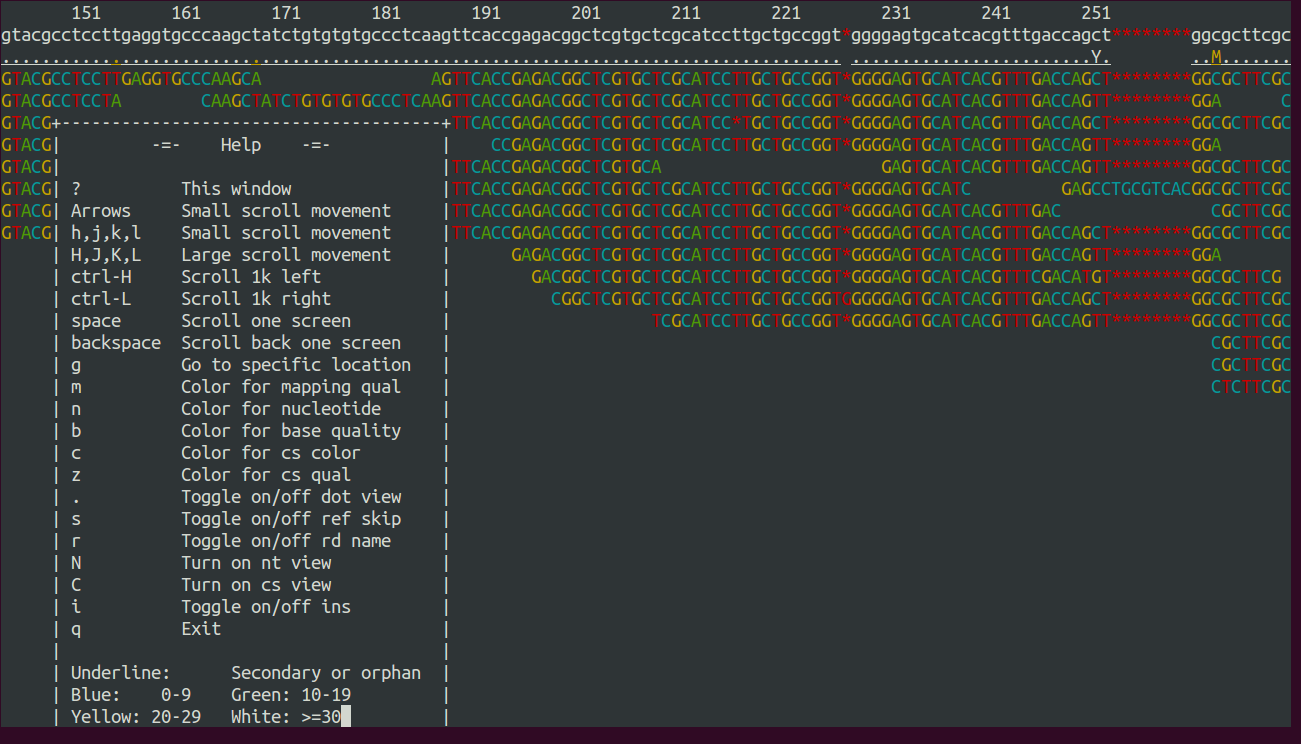
\includegraphics[width=14.5cm]{tview.png}
\caption{\label{fig:tview}Screenshot of tview}
\end{figure}

\clearpage
\subsection{IGV: viewer with a graphical user interface}
\label{sec-3-2}
I bet that many of you prefer to look at the alignment in a graphical
user interface. A decent free alignment viewer is \href{https://www.broadinstitute.org/igv/}{igv}, the Integrative
Genomics Viewer (see Fig. \ref{fig:igv} for a screenshot). Once you have
registered, you can launch the program with Java Web Start. We can't
promise that this works well in the course, since everything that
relies on a graphical user interface can be quite slow when using a
remote connection. Thus, you might want to download the required files
(deduplicated SAM file and reference genome) and try out igv on your
private computer. The interface is pretty much self-explanatory. To
look at the alignment, you first need to load a genome and then add
the mapped, sorted and indexed bam file.



\begin{figure}[htb]
\centering
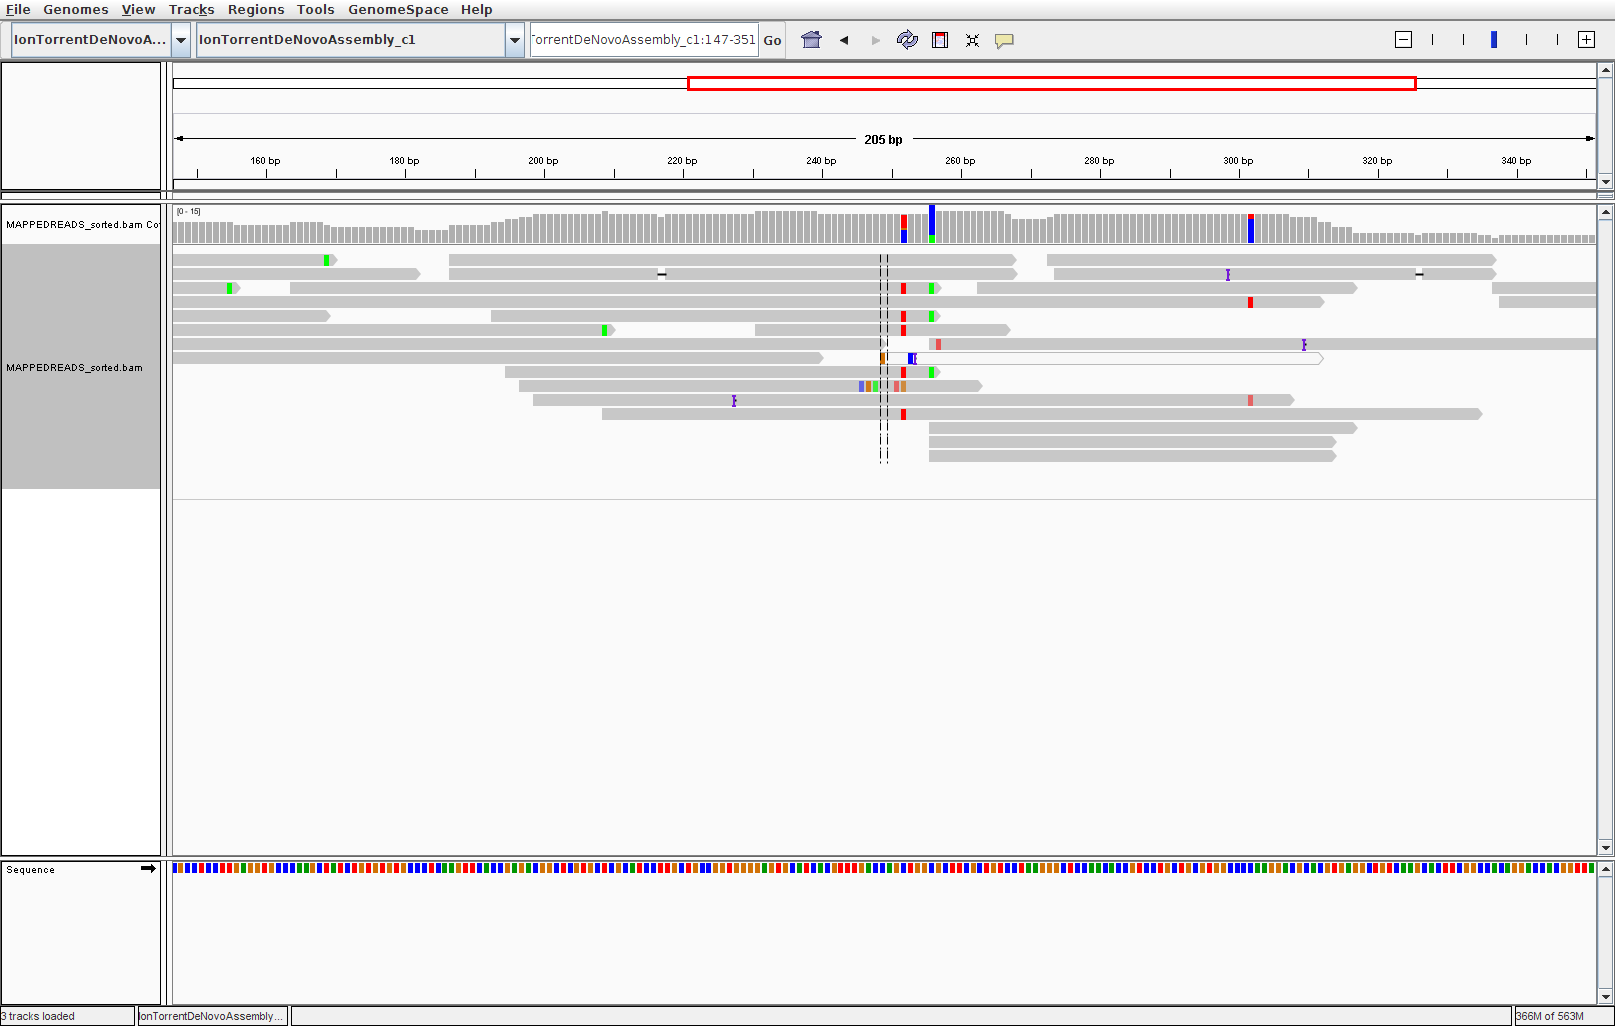
\includegraphics[width=17cm]{igv.png}
\caption{\label{fig:igv}Screenshot of igv with reads aligned to a reference and colored mismatches}
\end{figure}

\clearpage
\section{BONUS: SNP calling with samtools mpileup and bcftools}
\label{sec-4}
Given sequences aligned to a reference it seems that it should be trivial to
identify sequence variants. Surely any mismatches between the reference (in this case our assembly)
and reads is evidence for the
presence of a sequence variant. However, if the probability of observing a
sequencing error is larger than the frequency of sequence variants within the
population (an individual can be considered as a population of
two haploid genomes) then most sequence mismatches will be caused by
sequencing errors. This is usually the case (and overwhelmingly so) when looking at individuals from
within a single species and in order to identify a position as a sequence
variant we need to have more than one read diverging from the reference. How
many reads are required depends on the total number of reads, the qualities
of those reads and the expected variant frequency. If we are sequencing
populations, then we also have to consider the rarity of a given allele;
the rarer the allele one wishes to discover the larger the sequencing coverage
required. This has led to the
development of a rather large number of variant detection algorithms and
programs (see
\href{http://www.nature.com/nrg/journal/v15/n11/fig_tab/nrg3803_T3.html}{table 3} of \href{http://www.nature.com/nrg/journal/v15/n11/full/nrg3803.html}{Schlotterer \emph{et al}} for a list), and the difficulty of balancing
computation times, sensititivy and accuracy makes it likely that more methods
and or implementations will be written.

Here we will use the \texttt{samtools mpileup} in conjuction with 
\texttt{bcftools}. Computationally these are some of the simplest ways to detect variants
and are widely used. For more in depth analyses we would recommend that you
consider using other tool sets that have the potential to provide more
accurate variant detection at the cost of more processing time.

The tool \texttt{samtools mpileup} defaults to creating a pileup file, which summarizes aligned
base calls in text format (See \href{http://samtools.sourceforge.net/samtools.shtml}{here} for an overview of its options, and here for a detailed characterization of
a pileup file \url{http://samtools.sourceforge.net/pileup.shtml}). If you
call \texttt{samtools mpileup} with the \texttt{-u} or \texttt{-g} option the
output format is a vcf or bcf (compressed binary version of vcf) file;
vcf stands for 'variant call format'. Its format specifications are
described \href{https://samtools.github.io/hts-specs/VCFv4.2.pdf}{here} and summarized in Fig. \ref{fig:vcf}.

The first step for calling SNPs from your aligned and deduplicated
reads is:

\begin{minted}[fontsize=\scriptsize,bgcolor=lightgray,linenos]{sh}
samtools mpileup -g \
-f \
IonTorrentDeNovoAssembly_out.unpadded.fasta \
-q 20 \
-Q 20 \
-t DP \
-t SP \
MAPPEDREADS_dedup.bam  > MAPPEDREADS_dedup.bcf
\end{minted}

The chosen options are described on this \href{http://samtools.sourceforge.net/samtools.shtml}{page}. By setting the \texttt{-t SP} and
\texttt{-t DP} tags, samtools mpileup provides:

\begin{description}
\item[{\texttt{-t SP}}] per-sample Phred-scaled strand bias P-value
\item[{\texttt{-t DP}}] per sample read depth
\end{description}


To call SNPs from the bcf file, we use bcftools:

\begin{minted}[fontsize=\scriptsize,bgcolor=lightgray,linenos]{sh}
bcftools call -vm -V indels MAPPEDREADS_dedup.bcf >  MAPPEDREADS_variants.vcf
\end{minted}


Options:
\begin{description}
\item[{\texttt{-v}}] Output variant sites only
\item[{\texttt{-V indels}}] Skip indels
\item[{\texttt{-m}}] model for multiallelic and rare-variant calling
\end{description}


\begin{figure}[htb]
\centering
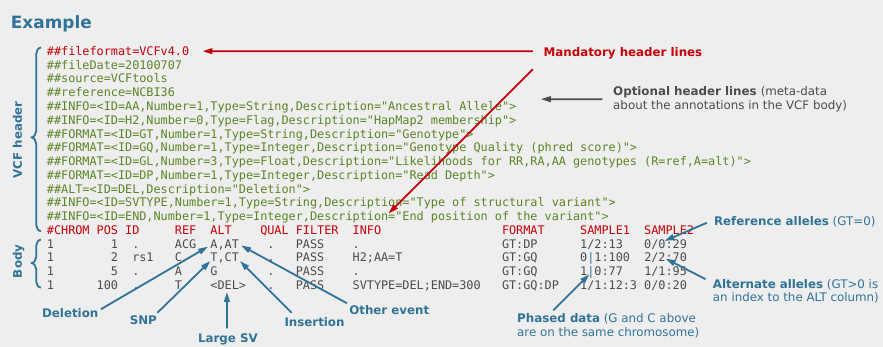
\includegraphics[width=17cm]{DanecekVcfFile.png}
\caption{\label{fig:vcf}VCF file overview from \href{http://vcftools.sourceforge.net/VCF-poster.pdf}{Petr Danecek}}
\end{figure}



To count how many SNPs were found, use the following command:

\begin{minted}[fontsize=\scriptsize,bgcolor=lightgray,linenos]{sh}
grep -v -c '^#' MAPPEDREADS_variants.vcf
\end{minted}

The option \texttt{-v} in combination with \texttt{\textasciicircum{}\#} excludes all header lines
that start with (\texttt{\textasciicircum{}}) the \texttt{\#}-sign. With the \texttt{-c} option, grep counts
the lines instead of writing them out.


To filter out SNPs that are low quality or covered by low depth, we
can use the \texttt{vcfutils.pl varFilter} that comes with samtools:

\begin{minted}[fontsize=\scriptsize,bgcolor=lightgray,linenos]{sh}
vcfutils.pl varFilter -d 5 -w 3 -Q 20  MAPPEDREADS_variants.vcf > MAPPEDREADS_variants_filtered.vcf
\end{minted}


Options used:
\begin{description}
\item[{\texttt{-d 5}}] minimum read depth of 5
\item[{\texttt{-w 3}}] SNP within 3 bp around a gap to be filtered. This may be
an alternative solution to re-alignment around indels
\item[{\texttt{-Q 20}}] minimum mapping quality of 20
\end{description}

Another useful option can be:
\begin{description}
\item[{\texttt{-1 0.0001}}] min P-value for strand bias (given the PV4-tag in the
vcf file). We obtained the PV4-tag by setting the \texttt{-t SP} tag in
\texttt{samtools mpileup}. This option filters out the SNPs that have a
strong strand-bias: SNPs that are supported by one strand and not
the other.
\end{description}


Count how many SNPs are left after filtering

\begin{minted}[fontsize=\scriptsize,bgcolor=lightgray,linenos]{sh}
grep -v -c '^#' MAPPEDREADS_variants_filtered.vcf
\end{minted}

The SNPs can be visualized with IGV. For this, we first need to
compress and index the vcf files: 

\begin{minted}[fontsize=\scriptsize,bgcolor=lightgray,linenos]{sh}
bgzip -c \
MAPPEDREADS_variants_filtered.vcf \
> MAPPEDREADS_variants_filtered.vcf.gz

tabix \
-p vcf \
MAPPEDREADS_variants_filtered.vcf.gz
\end{minted}

Open IGV and load the indexed bam file and the indexed vcf file.
Emacs 24.5.1 (Org mode 8.3beta)
\end{document}